\section{Person Isolation}
This section details the implementation of the person isolation methods described in Section \ref{design:person isolation}.\\

\subsection{Colour Based Isolation}
\label{imp:colour based isolation}
Figure \ref{fig:colour based cut off} shows the colour based isolation, described in Section \ref{design:colour based isolation}. As originally suspected, when implemented this method appears to perform well, removing all non-person details from the scene.\\

\begin{figure}[h]
    \begin{center}
        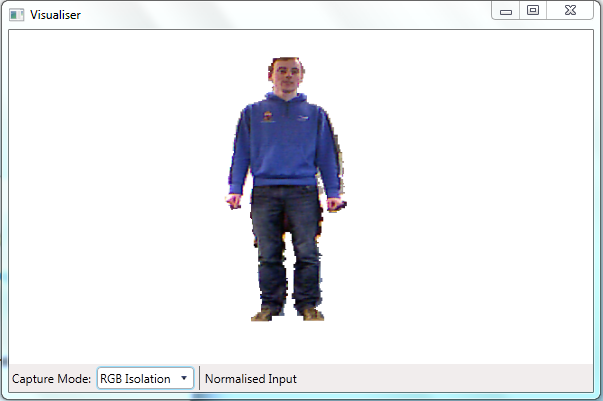
\includegraphics[scale=0.4]{images/parse4} 
    \end{center}
    \caption{Colour based isolation.}
    \label{fig:colour based cut off}
\end{figure} 

However, colour based isolation is not immediately useful as depth data is need to create the point cloud.\\ 

An attempt to overcome this was to try to map the colour pixels, which corresponded to a person, to depth pixels. Unfortunately, as the depth sensor and colour camera are not situated in the same place on the Kinect, see Figure \ref{fig:kinectoffset}, this mapping is non trivial and is currently an open problem in and of itself in the Kinect development community. Efforts were devoted by the group to fix or at least account for this problem, however none of the solutions proposed lead to a sufficiently isolated person. In Figure \ref{fig:a poorly isolated person}, it can be seen that colour based isolation leads to a poorly isolated person in depth space. The lack of effective mapping between colour and depth pixels also negated the possibility of a textured point cloud being displayed by the toolkit.\\

\begin{figure}[h]
\begin{center}
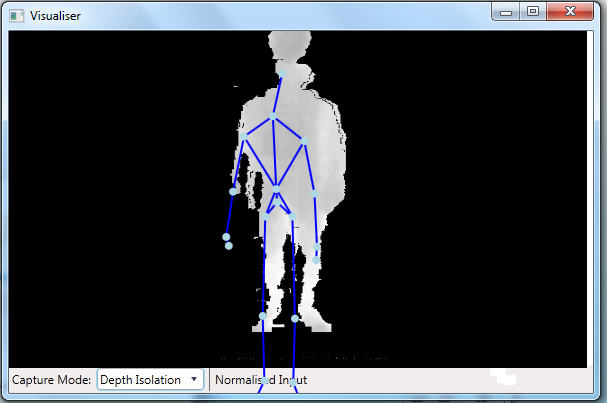
\includegraphics[scale=0.4]{images/parse5} 
\end{center}
\caption{A poorly isolated person.}
\label{fig:a poorly isolated person}
\end{figure} 

\subsection{Depth Based Isolation}
\label{imp:depth based isolation}
Figure \ref{fig:depth based cut off} shows the depth based isolation, described in Section \ref{design:depth based isolation}. As predicted, this cut appears to be sufficient to eliminate a large proportion of non-person data but does not remove the ring of points at the same depth as the person.\\

\begin{figure}[h]
\begin{center}
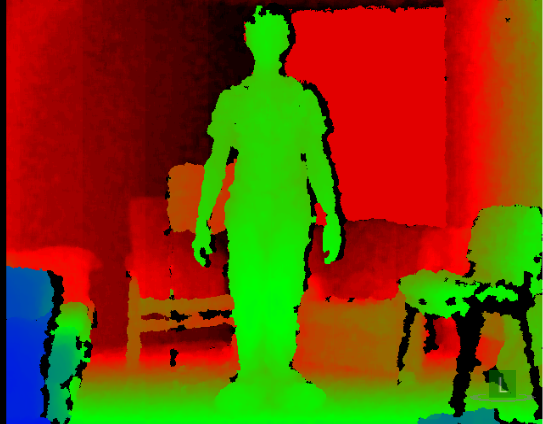
\includegraphics[scale=0.4]{images/parse1} 
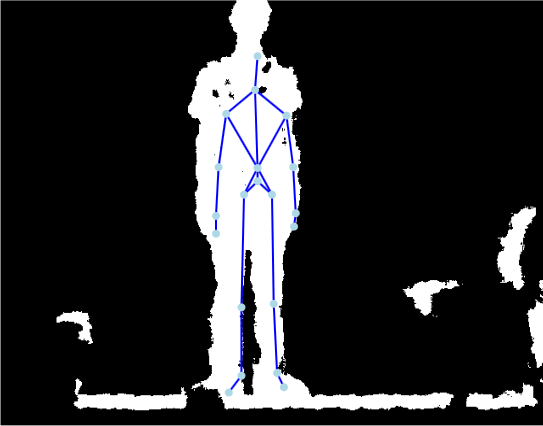
\includegraphics[scale=0.4]{images/parse2}
\end{center}
\caption{Depth based cut off, before (left) and after (right).}
\label{fig:depth based cut off}
\end{figure} 

Figure \ref{fig:depth and hand based cut off} hand based extension to the depth cut off. As predicted, the combination of using depth and hand position appears sufficient to isolate a person, although the floor beneath them does remain. As such, this method was chosen to isolate the person. To aid the creation of a point cloud, the isolated person is coloured from black to white as depth increases away from the camera.\\

\begin{figure}[h]
\begin{center}
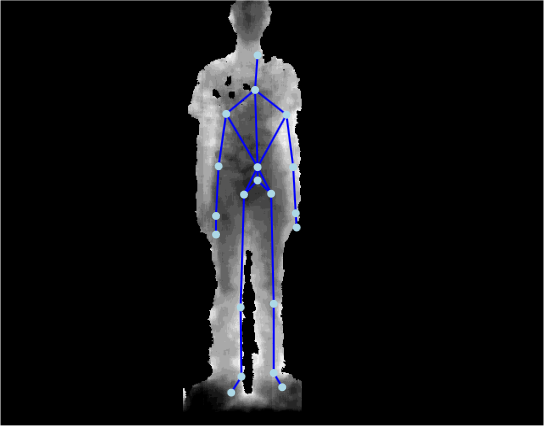
\includegraphics[scale=0.4]{images/parse3} 
\end{center}
\caption{Depth and hand based cut off, with colouring.}
\label{fig:depth and hand based cut off}
\end{figure} 